\section{Decoupling for the paraboloid}
The Fourier decoupling inequality is a kind of $L^{p}$ orthogonality statement for functions with Fourier support close to the paraboloid $\mathbb{P} = \Set{ (\xi,\abs{\xi}^{2}) \given \xi\in\R^{d} }$.
Some of its far-reaching applications will be discussed later on.
It was originally proved in \cite{MR3374964}.
Our presentation is based on the simplified proofs in \cite{MR3592159} and \cite{arxiv:1902.03450}.

For inductive purposes it is convenient to formulate the Fourier support condition in a way that is invariant under affine transformations that preserve the paraboloid.
We will consider functions with Fourier support inside parallelepipeds adapted to the paraboloid $\mathbb{P}$.
Figure~\ref{fig:Fourier-supp} shows the parallelepipeds of scales $2^{-1}$, $2^{-2}$, and $2^{-3}$, respectively, inside the parallelepiped of scale $2^{0}$ (in the case $d=1$).
The picture is self-similar: inside each parallelepiped of a given scale there are $2^{d}$ parallelepipeds, and any parallelepiped can be mapped onto any other by an affine transformation that preserves the collection of all parallelepipeds.
\newcommand{\figparabolicscaling}[1]{
\begin{scope}[black,cm={0.5,0,0,0.25,(0,0)}]
#1
\end{scope}
\begin{scope}[black,cm={0.5,0.5,0,0.25,(0.5,0.25)}]
#1
\end{scope}
}
\newcommand{\figunitball}{\draw (-1.5,-1.5) rectangle (1.5,1.5);}
\begin{figure}\label{fig:Fourier-supp}
\begin{center}
\begin{tabular}{ccc}
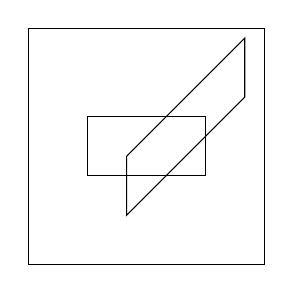
\begin{tikzpicture}
\figunitball
\figparabolicscaling{\figunitball}
\end{tikzpicture} &
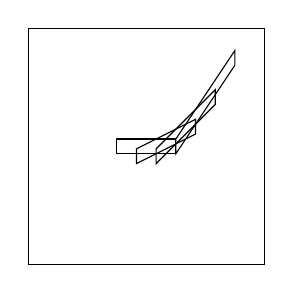
\begin{tikzpicture}
\figunitball
\figparabolicscaling{\figparabolicscaling{\figunitball}}
\end{tikzpicture} &
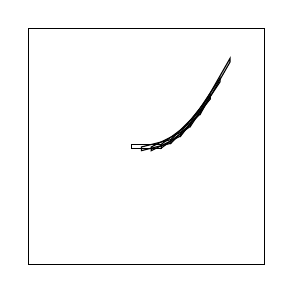
\begin{tikzpicture}
\figunitball
\figparabolicscaling{\figparabolicscaling{\figparabolicscaling{\figunitball}}}
\end{tikzpicture}
\end{tabular}
\end{center}
\caption{Fourier support parallelepipeds at scales $2^{-1},2^{-2},2^{-3}$}
\end{figure}

We proceed with a more formal description.
A \emph{dyadic cube} (of side length $\delta$) is a cube of the form $\delta (a + [0,1]^{d})$ with $a \in \Z^{d}$ and $\delta$ a power of $2$.
We will denote by $\Part[Q]{\delta}$ the partition of a dyadic cube $Q$ into dyadic cubes with side length $\delta$ ($\delta$ must be smaller than the side length of $Q$ for this to make sense).
We omit $Q$ from the notation $\Part[Q]{\delta}$ if $Q=[0,1]^{d}$.

For $\theta = a + \delta [0,1]^{d} \in \Part{\delta}$ we will denote by $f_{\theta}$ an arbitrary function of the form $M_{\theta}f$, where $f \in L^{p}(\R^{d+1})$ with $\supp \widehat{f} \subset [-2,2]^{d+1}$ and
\begin{equation}\label{eq:parabolic-scaling}
M_{\theta}f(x,y) = e(a\cdot x + \abs{a}^{2} y) (f \circ L_{\theta})(x,y),
\quad
x\in\R^{d}, y\in\R,
\end{equation}
where $L_{\theta}$ is the linear transformation
\[
L_{\theta} =
\begin{pmatrix}
\delta I_{d} & 0\\
0 & \delta^{2}
\end{pmatrix}
\begin{pmatrix}
I_{d} & (2a_{1},\dotsc,2a_{d})^{T}\\
0 & 1
\end{pmatrix}.
\]
and $I_{d}$ denotes the identity $d\times d$ matrix.
Equivalently, $f_{\theta}$ denotes an arbitrary $L^{p}$ function with the Fourier support condition
\begin{equation}
\label{eq:Fourier-support}
\supp \widehat{f_{\theta}}
\subseteq
(a,\abs{a}^{2}) + L_{\theta}^{*}([-2,2]^{d+n}).
\end{equation}
\noindent\fbox{\parbox{\textwidth}{Roughly speaking, $\supp \widehat{f_{\theta}}$ is contained in a box of size $\delta \times \dotsm \times \delta \times \delta^{2}$ that contains the part of paraboloid over $\theta$.}}

For $1 \leq p,q \leq \infty$ and $\delta>0$, let the \emph{$\ell^{q}L^{p}$ decoupling constant} $\Dec_{d}^{p,q}(\delta)$ be the smallest constant such that the inequality
\begin{equation}\label{eq:dec-const}
\norm[\big]{\sum_{\theta \in \Part{\delta}} f_{\theta}}_{L^p}
\le
\Dec_{d}^{p,q}(\delta) (\sum_{\theta} \norm{f_{\theta}}_{L^p}^q)^{1/q}
\end{equation}
holds for any functions $f_{\theta}$ as above.
The main decoupling estimate is the following.
\begin{theorem}[{\cite{MR3374964}}]\label{thm:dec-paraboloid}
Let $d \geq 1$ and $2 \leq p \leq \infty$.
Then for every $\epsilon>0$ we have
\begin{equation}\label{eq:dec-paraboloid}
\Dec_{d}^{p,2}(\delta)
\lesssim_{\epsilon}
\begin{cases}
\delta^{-\epsilon}, & 2 \leq p \leq 2(d+2)/d,\\
\delta^{-d/2+(d+2)/p-\epsilon}, & 2(d+2)/d < p \leq \infty.
\end{cases}
\end{equation}
\end{theorem}
\begin{remark}
This is a comment on numerology, or the exponents in \eqref{eq:dec-paraboloid}.
For $p=2$ and $p=\infty$ the inequality \eqref{eq:dec-paraboloid} holds even with $\epsilon = 0$.
For $p=2$ this follows from Plancherel's theorem, and for $p=\infty$ from the triangle inequality.
By a complex interpolation argument that is explained in Section~\ref{sec:dec-interpolation} it will suffice to consider the endpoint $p=2(d+2)/d$ to obtain the inequality \eqref{eq:dec-paraboloid} for all $2 \leq p \leq \infty$.
\end{remark}


\subsection{Optimatity of the decoupling inequality}\label{sec:sharpness}
In this section we show that the estimates in Theorem~\ref{thm:dec-paraboloid} are essentially optimal.

\begin{example}
Consider first $f_{\theta} = M_{\theta} f$, where $f$ is a fixed Schwartz function with $f(0)=1$ and $\hat{f}$ supported in the unit cube.
Then by scaling $\norm{f_{\theta}}_{p} \sim \delta^{-(d+2)/p}$.
On the other hand, $\Re f_{\theta} \gtrsim 1$ on a fixed neigborhood of $0$.
Hence
\[
\norm[\big]{ \sum_{\theta \in \Part{\delta}} f_{\theta} }_{p} \gtrsim \abs{\Part{\delta}} \sim \delta^{-d},
\]
and it follows that
\[
\Dec_{d}^{p,q}(\delta) \gtrsim \delta^{-d+\frac{d}{q}+\frac{d+2}{p}}.
\]
For $q=2$ and $p>2(d+2)/d$ this is the exponent in \eqref{eq:dec-paraboloid} (up to the $\epsilon$ loss).
\end{example}

\begin{example}
Consider next $f_{\theta}(x,y)=\eta(\delta^{2} (x,y)) e(a \cdot x + \abs{a}^{2} y)$, where $\eta$ is a Schwartz function with $\hat\eta$ supported in the unit cube and $a \in \theta$.
Then $\norm{f_{\theta}}_{p} \sim \delta^{-2(d+1)/p}$ and by H\"older's inequality with $2 \leq p \leq \infty$ and orthogonality
\begin{multline*}
\delta^{-2(d+1)(\frac12-\frac1p)} \norm{\sum_{\theta \in \Part{\delta}} f_{\theta}}_{p}
\sim
\norm{\eta(\delta^{2}\cdot)}_{\frac{1}{1/2-1/p}} \norm{\sum_{\theta \in \Part{\delta}} f_{\theta}}_{p}
\geq
\norm{\sum_{\theta \in \Part{\delta}} \eta(\delta^{2}\cdot) f_{\theta}}_{2}\\
\gtrsim
\bigl( \sum_{\theta \in \Part{\delta}} \norm{\eta(\delta^{2}\cdot) f_{\theta}}_{2}^{2} \bigr)^{1/2}
\sim
\delta^{-d/2}\delta^{-2(d+1)/2}.
\end{multline*}
It follows that
\[
\Dec_{d}^{p,q}(\delta) \gtrsim \delta^{\frac{d}{q}-\frac{d}{2}}
\]
for $2 \leq p \leq \infty$, and in the case $q=2$ and $2 \leq p \leq 2(d+2)/d$ this is exacly the exponent in \eqref{eq:dec-paraboloid} (up to the $\epsilon$ loss).
\end{example}

\begin{example}
Finally, consider again the functions in the first example and translate them so that they become essentially disjointly supported.
Then
\[
\norm[\big]{\sum_{\theta \in \Part{\delta}} f_{\theta}}_{L^p}
\approx
(\sum_{\theta \in \Part{\delta}} \norm{f_{\theta}}_{L^p}^p)^{1/p}
\approx
\abs{\Part{\delta}}^{1/p-1/q} (\sum_{\theta \in \Part{\delta}} \norm{f_{\theta}}_{L^p}^q)^{1/q},
\]
so
\[
\Dec_{d}^{p,q}(\delta) \gtrsim \delta^{d/q-d/p}.
\]
This shows that we cannot expect any estimates for $p<q=2$ other than those that follow by interpolation between orthogonality at $p=2$ and Minkowski's inequality at $p=1$.
\end{example}

\begin{remark}
It is known from \cite[p.~118]{MR1209299} that the $\epsilon$ loss in \eqref{eq:dec-paraboloid} cannot be completely removed in general.
On the other hand, the precise dependence on $\delta$ in \eqref{eq:dec-paraboloid} has not been quantified except in the case $d=1$ \cite{arxiv:1711.01202}.
\end{remark}


\subsection{Basic properties of the decoupling constant}
\subsubsection{Parabolic scaling}\label{sec:parabolic-scaling}
We use functions of the form \eqref{eq:parabolic-scaling} in order to make explicit a scaling invariance of the decoupling inequality.
If $\delta_{0},\delta_{1} \leq 1$ are powers of $2$ and $\theta_{0} \in \Part{\delta_{0}}$, then there is a natural bijection between $\Part{\delta_{1}}$ and $\Part[\theta_{0}]{\delta_{0}\delta_{1}}$ given by the composition of translation ans scaling that maps $[0,1]^{d}$ to $\theta$.
Moreover, if $\theta$ is mapped to $\theta'$ be this bijection, then $M_{\theta'} = M_{\theta_{0}} \circ M_{\theta}$, so we can write $f_{\theta'} = M_{\theta_{0}} \tilde{f}_{\theta}$.
Hence
\begin{align*}
\norm[\big]{\sum_{\theta' \in \Part[\theta_{0}]{\delta_{0}\delta_{1}}} f_{\theta'}}_{p}
&=
\norm[\big]{M_{\theta_{0}} \sum_{\theta \in \Part{\delta_{1}}} \tilde{f}_{\theta}}_{p}\\
&=
\delta_{0}^{-(d+2)/p} \norm[\big]{\sum_{\theta \in \Part{\delta_{1}}} \tilde{f}_{\theta}}_{p}\\
&\leq
\delta_{0}^{-(d+2)/p} \Dec_{d}^{p,q}(\delta_{1}) \bigl( \sum_{\theta \in \Part{\delta_{1}}} \norm{ \tilde{f}_{\theta} }_{p}^q \bigr)^{1/q}\\
&=
\Dec_{d}^{p,q}(\delta_{1}) \bigl( \sum_{\theta \in \Part{\delta_{1}}} \norm{ M_{\theta_{0}} \tilde{f}_{\theta} }_{p}^q \bigr)^{1/q}\\
&=
\Dec_{d}^{p,q}(\delta_{1}) \bigl( \sum_{\theta' \in \Part[\theta_{0}]{\delta_{0}\delta_{1}}} \norm{ \tilde{f}_{\theta'} }_{p}^q \bigr)^{1/q}.
\end{align*}


\subsubsection{Larger Fourier support}\label{sec:dec-larger-Fourier-supp}
The choise of the Fourier support condition $\supp \widehat{f} \subset [-2,2]^{d}$ in $f_{\theta} = M_{\theta} f$ is not particularly important.
In particular, for functions of the form $f_{\theta} = M_{\theta} f$ with $\supp \widehat{f} \subset [-C,C]^{d}$ we obtain
\begin{equation}\label{eq:dec-larger-Fourier-support}
\norm[\big]{\sum_{\theta \in \Part{\delta}} f_{\theta}}_{L^p}
\lesssim
\Dec_{d}^{p,q}(C\delta) (\sum_{\theta} \norm{f_{\theta}}_{L^p}^q)^{1/q}.
\end{equation}
This is because such $f_{\theta}$ satisfy \eqref{eq:Fourier-support} with a larger dyadic cube (of scale $\leq C\delta$).

\subsubsection{Interpolation}\label{sec:dec-interpolation}
Let $1 \leq p_{0},p_{1},q_{0},q_{1} \leq \infty$ and $0 < \eta < 1$.
Define $p_{\eta},q_{\eta}$ by
\[
\frac{1}{p_{\eta}} = \frac{1-\eta}{p_{0}} + \frac{\eta}{p_{1}},
\quad
\frac{1}{q_{\eta}} = \frac{1-\eta}{q_{0}} + \frac{\eta}{q_{1}}.
\]
Then we have
\begin{equation}\label{eq:dec-interpolation}
\Dec_{d}^{p_{\eta},q_{\eta}}(\delta)
\lesssim
\Dec_{d}^{p_{0},q_{0}}(4\delta)^{1-\eta} \Dec_{d}^{p_{1},q_{1}}(4\delta)^{\eta}.
\end{equation}
This would follow from complex interpolation if we could disregard the Fourier support restrictions, which is of course impossible.
In order to apply a standard complex interpolation result we have to reformulate the decoupling inequality~\eqref{eq:dec-const} as an estimate for a linear operator on an $\ell^{q}L^{p}$ space.
To this end let $\psi$ be a smooth function on $\R^{d+1}$ with $\one_{[-2,2]^{d+1}} \leq \psi \leq \one_{[-4,4]^{d+1}}$.
Define the multiplier operator $\widehat{Tf} := \psi \widehat{f}$.
Since this is a convolution operator with kernel $\check{\psi} \in L^{1}(\R^{d+1})$, it is bounded on any $L^{p}$ space with $1 \leq p \leq \infty$.
It follows that the operators $T_{\theta} := M_{\theta} T M_{\theta}^{-1}$ are bounded uniformly for all dyadic cubes $\theta$.
On the other hand, for an arbitrary function $g \in L^{p}(\R^{d+1})$ the function $T_{\theta} g$ satisfies the support condition in Section~\ref{sec:dec-larger-Fourier-supp}.
It follows that for arbitrary functions $g_{\theta} \in L^{p}(\R^{d+1})$ we have
\[
\norm[\big]{\sum_{\theta \in \Part{\delta}} T_{\theta} g_{\theta}}_{p}
\lesssim
\Dec_{d}^{p,q}(4\delta) (\sum_{\theta} \norm{T_{\theta} g_{\theta}}_{p}^q)^{1/q}
\lesssim
\Dec_{d}^{p,q}(4\delta) (\sum_{\theta} \norm{g_{\theta}}_{p}^q)^{1/q},
\]
where we have used~\eqref{eq:dec-larger-Fourier-support} and the uniform boundedness of the operators $T_{\theta}$.
This is now an $\ell^{q}(\Part{\delta},L^{p}(\R^{d+1})) \to L^{p}(\R^{d+1})$ bound for the linear operator $(g_{\theta})_{\theta} \mapsto \sum_{\theta} T_{\theta} g_{\theta}$.
By complex interpolation we obtain
\[
\norm[\big]{\sum_{\theta \in \Part{\delta}} T_{\theta} g_{\theta}}_{p_{\eta}}
\lesssim
\Dec_{d}^{p_{0},q_{0}}(4\delta)^{1-\eta} \Dec_{d}^{p_{1},q_{1}}(4\delta)^{\eta}
(\sum_{\theta} \norm{g_{\theta}}_{p_{\eta}}^{q_{\eta}})^{1/q_{\eta}}.
\]
On the other hand, for $f_{\theta}$ satisfying the standing Fourier support condition we have $T_{\theta}f_{\theta}=f_{\theta}$, and this implies \eqref{eq:dec-interpolation}.

\subsection{Localization}\label{sec:dec-local}
The freedom to enlarge the Fourier support in Section~\ref{sec:dec-larger-Fourier-supp} can be used to localize decoupling inequalities.
Let $\eta$ be a positive Schwartz function on $\R^{d+1}$ such that $\supp \hat{\eta} \subset B(0,c)$ and $\eta \geq 1$ on $B(0,1)$.
Let $B = B(x,\delta^{-2}) \subset \R^{d+1}$ be a ball of radius $\delta^{-2}$ centered at $x$ and $\eta_{B} := \eta(\delta^{2}(\cdot-x))$.
Then the functions $f_{\theta}\eta_{B}$ are as in Section~\ref{sec:dec-larger-Fourier-supp}, so we obtain
\begin{equation}\label{eq:dec-local:com-F-supp-cutoff}
\norm[\big]{\sum_{\theta \in \Part{\delta}} f_{\theta} \eta_{B}}_{p}
\lesssim
\Dec_{d}^{p,q}(C\delta) \bigl( \sum_{\theta} \norm{\eta_{B} f_{\theta}}_{p}^q \bigr)^{1/q}.
\end{equation}
It is sometimes convenient to use other kinds of weights.
For a ball $B=B(c_B, r_B)\subset \R^{d+1}$ and $E>d+1$, define an associated weight
\begin{equation}\label{eq:w_B}
w_{B, E}(x):=\Bigl( 1+\frac{\abs{x-c_B}}{r_B} \Bigr)^{-E}.
\end{equation}
The exponent $E$ will not be important and will be usually omitted from the notation.

From the estimate \eqref{eq:dec-local:com-F-supp-cutoff} and using $\one_{B} \leq \eta_{B} \lesssim w_{B}$ we immediately obtain
\[
\norm[\big]{\sum_{\theta \in \Part{\delta}} f_{\theta} }_{L^{p}(B)}
\lesssim
\Dec_{d}^{p,q}(C\delta) \bigl( \sum_{\theta} \norm{f_{\theta}}_{L^{p}(w_{B})}^q \bigr)^{1/q}
\]
for balls $B$ of radius $R^{2}$.
It is inconvenient that the weights on the left-hand and the right-hand side differ.
This can be remedied by the averaging argument in Lemma~\ref{lem:1-w} below, and the following estimate can be obtained for $q \leq p$.
\begin{equation}\label{eq:dec-local:w_B}
\norm[\big]{\sum_{\theta \in \Part{\delta}} f_{\theta}}_{L^p(w_{B})}
\lesssim
\Dec_{d}^{p,q}(\delta) (\sum_{\theta} \norm{f_{\theta}}_{L^p(w_{B})}^q)^{1/q}.
\end{equation}
Similarly we can localize the rescaled decoupling inequality in Section~\ref{sec:parabolic-scaling} to balls of size $(\delta_{0}\delta_{1})^{-2}$.

\subsubsection{Power weights}\label{sec:cutoff}
A key property of the weights \eqref{eq:w_B} is the inequality
\begin{equation}
\label{eq:1-w}
\one_B
\lesssim
\sum_{B' \in \calB(B,R)} w_{B'}
\lesssim
w_B
\end{equation}
that holds for all balls $B \subset \R^{n}$ and all $0<R$ that are smaller than the radius of $B$.
Here and later $\calB(B,R)$ denotes a boundedly overlapping covering of a set $B$ by balls of radius $R$.
The implicit constants in \eqref{eq:1-w} do not depend on $B$ and $R$.

The following result allows to deduce inequalities for $L^{p}(w_{B})$ norms from inequalities for $L^{p}(\one_{B})$ norms.
It is necessitated by the fact that inequalities converse to \eqref{eq:1-w} do not hold.
\begin{lemma}[{\cite[Lemma 4.1]{MR3592159}}]
\label{lem:1-w}
Let $\calW$ be the collection of all weights, that is, positive, integrable functions on $\R^n$.
Fix $R>0$ and $E>n$.
Let $O_1,O_2 : \calW\to[0,\infty]$ be any functions with the following properties.
\begin{enumerate}
\item\label{it:O:1<w} $O_1(\one_B)\leq O_2(w_{B,E})$ for all balls $B\subset \R^n$ with radius $R$
\item\label{it:O:subadd} $O_1(\alpha u+\beta v)\le \alpha O_1(u)+\beta O_1(v)$, for each $u,v\in\calW$ and $\alpha,\beta > 0$
\item\label{it:O:supadd} $O_2(\alpha u+\beta v)\ge \alpha O_2(u)+\beta O_2(v)$, for each $u,v\in\calW$ and $\alpha,\beta > 0$
\item\label{it:O:monotone} If $u\le v$ then $O_i(u)\le O_i(v)$.
\item\label{it:O:continuous} If $(u_{j})_{j} \subset \calW$ is a monotonically increasing sequence with $u_{j} \to u \in \calW$ pointwise almost everywhere, then $O_1(u) = \lim_{j} O_1(u_{j})$.
\end{enumerate}
Then for each ball $B \subset \R^{n}$ with radius $R$ we have
\[
O_1(w_{B,E})
\lesssim_{n,E}
O_2(w_{B,E})
\]
The implicit constant depends only on $n$ and $E$.
\end{lemma}

\begin{proof}
Let $\calB := \calB(\R^n,R)$.
Note that
\[
w_B(x)
\leq
C \sum_{B'\in\calB} w_B(c_{B'}) \one_{B'}(x)
\]
and that
\[
\sum_{B'\in\calB}w_{B'}(x)w_B(c_{B'})
\leq
C w_B(x)
\]
for a sufficiently large constant $C=C(n,E)>0$.
Hence
\begin{align*}
O_{1}(w_{B})
&\leq
\sup_{\calB' \subset \calB \ \textrm{finite}} O_{1}\bigl( C \sum_{B'\in\calB'} w_B(c_{B'}) \one_{B'} \bigr)
&\text{by \eqref{it:O:continuous}}\\
&\leq
\sup_{\calB' \subset \calB \ \textrm{finite}} C \sum_{B'\in\calB'} w_B(c_{B'}) O_{1}( \one_{B'} )
&\text{by \eqref{it:O:subadd}}\\
&\leq
C \sup_{\calB' \subset \calB \ \textrm{finite}} \sum_{B'\in\calB} w_B(c_{B'}) O_{2}(w_{B'})
&\text{by \eqref{it:O:1<w}}\\
&\leq
C^{2} \sup_{\calB' \subset \calB \ \textrm{finite}} O_{2}\bigl( C^{-1} \sum_{B'\in\calB} w_{B'} w_B(c_{B'}) \bigr)
&\text{by \eqref{it:O:supadd}}\\
&\leq
C^{2} O_{2}(w_{B}).
&\text{by \eqref{it:O:monotone}}
&\qedhere
\end{align*}
\end{proof}

\begin{remark}
\label{rem:1-w}
Lemma~\ref{lem:1-w} will be usually applied with functionals of the form
\begin{align}
O_1(v) &:= \norm{f}_{L^p(v)}^p \label{eq:O_1:practical}\\
O_2(v) &:= A (\sum_{i}\norm{f_i}_{L^p(v)}^{q})^{\frac{p}{q}}, \label{eq:O_2:practical}
\end{align}
where $1 \leq q \leq p$.
It is clear that conditions \eqref{it:O:subadd} and \eqref{it:O:monotone} hold for these choices.
The condition \eqref{it:O:supadd} follows from the reverse Minkowski inequality in $\ell_{\frac{q}{p}}$:
\begin{multline*}
O_2(v+w)
=
A \Bigl( \sum_{i} \bigl( \int \abs{f_{i}}^{p} v + \int \abs{f_{i}} w \bigr)^{q/p} \Bigr)^{p/q}\\
\geq
A \Bigl( \sum_{i} \bigl( \int \abs{f_{i}} v \bigr)^{q/p} \Bigr)^{p/q}
+
A \Bigl( \sum_{i} \bigl( \int \abs{f_{i}} w \bigr)^{q/p} \Bigr)^{p/q}
=
O_2(v) + O_2(w)
\end{multline*}
\end{remark}

\begin{remark}
We recall the proof of the reverse Minkowski inequality, which is basically identical to the proof of the direct Minkowski inequality.
Let $0<r\leq 1$ and let $f : X \times Y \to [0,\infty]$ be a function such that $0 < \norm{\int_{Y} f}_{L^{r}(X)} < \infty$.
Then by reverse H\"older inequality we have
\begin{multline*}
\int_{X} \abs[\big]{\int_{Y} f(x,y) \dif y}^{r} \dif x
=
\int_{Y} \int_{X} f(x,y') \abs[\big]{\int_{Y} f(x,y) \dif y}^{r-1} \dif x \dif y'\\
\geq
\int_{Y} \Bigl( \int_{X} f(x,y')^{r} \dif x \Bigr)^{1/r} \Bigl( \int_{X} \abs[\big]{\int_{Y} f(x,y) \dif y}^{r} \dif x \Bigr)^{1-1/r} \dif y'.
\end{multline*}
The reverse H\"older inequality is just the usual H\"older inequality in which one of the terms is brought to the other side.
Rearranging we obtain
\[
\Bigl( \int_{X} \abs[\big]{\int_{Y} f(x,y) \dif y}^{r} \dif x \Bigr)^{1/r}
\geq
\int_{Y} \Bigl( \int_{X} f(x,y')^{r} \dif x \Bigr)^{1/r} \dif y'.
\]
\end{remark}

\subsubsection{Reverse H\"older inequality}
We close this section with the following reverse H\"older inequality.
\begin{corollary}[{cf.\ \cite[Corollary 4.1]{MR3592159}}]
\label{cor:rev-holder}
For each $1 \leq t \leq p < \infty$, each $E>n$, each $R>0$ and $\delta>0$ with $R\delta \geq 1$, each function $f : \R^{n} \to \C$ with $\diam(\supp \hat{f}) \lesssim \delta$, and each ball $B \subset \R^n$ with radius $R$ we have
\begin{equation}
\label{eq:rev-holder}
\norm{f}_{\avL^p(w_{B,E})}
\lesssim
(R\delta)^{n/t-n/p}
\norm{f}_{\avL^t (w_{B,\frac{E t}{p}})},
\end{equation}
with the implicit constant independent of $R$, $\delta$, $B$, and $f$.
\end{corollary}
Here and later we denote normalized $L^{p}$ norms by
\begin{equation}
\label{eq:avL}
\norm{f}_{\avL^{p}(B)} := \abs{B}^{-1/p} \norm{f}_{L^{p}(B)},
\quad
\norm{f}_{\avL^{p}(w_{B})} := \abs{B}^{-1/p} \norm{f}_{L^{p}(w_{B})}.
\end{equation}
\begin{proof}
Let $\eta$ be a positive Schwartz function on $\R^n$ with $\one_{B(0,1)}\le \eta$ and such that $\supp (\widehat{\eta}) \subset B(0,1)$.
We can thus write
\[
\norm{f}_{L^p(B)}
\le
\norm{\eta_B f}_{L^p(\R^n)},
\]
where $\eta_{B}$ is an appropriate $L^{\infty}$-scaling and translation of $\eta$.
Let $\theta$ be a Schwartz function on $\R^{n}$ such that $\hat{\theta} = 1$ for $\abs{\theta} \leq 10$.
Since
\[
\diam(\supp \widehat{\eta_{B} f})
\leq
\diam(\supp \widehat{\eta_{B}}) + \diam(\supp \hat{f})
\lesssim
1/R + \delta
\lesssim
\delta,
\]
we have that
\[
\eta_B f
=
(\eta_B f)* \theta_B,
\]
where $\theta_{B}$ is an appropriate $L^{1}$-scaling and modulation of $\theta$.
By Young's convolution inequality with exponents
\[
\frac{1}p=\frac1{t}+\frac1{r}-1=\frac{1}{t}-\frac1{r'}
\]
we can write
\[
\norm{\eta_B f}_{L^p(\R^n)}
\le
\norm{\eta_B f}_{L^t(\R^n)} \norm{\theta_B}_{L^r(\R^n)}
\lesssim
\delta^{n/r'} \norm{f}_{L^t(\eta_B^{t})}.
\]
Rearranging this inequality and estimating $\eta_{B} \lesssim w_{B,E}^{1/p}$ we obtain
\[
\abs{B}^{-1/p} \norm{f}_{L^p(B)}
\lesssim_{n,E}
(R\delta)^{n/r'} \abs{B}^{-1/t} \norm{f}_{L^t(w_{B,E}^{t/p})}
\]
for any $E>0$.
Now we can apply Lemma~\ref{lem:1-w} with
\begin{align*}
O_{1}(v) &:= R^{-n} \int \abs{f}^{p} v,\\
O_{2}(v) &:= A (R\delta)^{n/t-n/p} R^{-n p/t} \Bigl( \int \abs{f}^{t} v^{t/p} \Bigr)^{p/t}.
\qedhere
\end{align*}
\end{proof}

\subsection{Linear versus multilinear decoupling}
\subsubsection{Transversality}\label{sec:gen:transverse}
One of the main advantages of the decoupling inequality \eqref{eq:dec-const} it can be reduced to the corresponding multilinear inequality involving transverse pieces of the paraboloid.
This is the objective of this Section~\ref{sec:gen:transverse}.
We fix $d\geq 1$, and if $d>1$ we assume that Theorem~\ref{thm:dec-paraboloid} is already known with $d$ replaced by $d-1$.
All constants are allowed to depend on $d$ and $p$, but not on other parameters unless indicated.

Recall that in the multilinear restriction theorem we called subsets $S_{1},\dotsc,S_{d+1}$ of a $d$-dimensional hypersurface in $\R^{d+1}$ \emph{$\nu$-transverse} if $\abs{N_{1} \wedge \dotsb \wedge N_{d+1}} > \nu$ for any unit normal vectors $N_{j}$ to $S_{j}$.
The same notion of transversality will be used here.
However, we also have to understand what it means in terms of the parametrization of the paraboloid $\mathbb{P}$ as the graph of $\Phi(\xi) = \abs{\xi}^{2}$ on the unit cube $[0,1]^{d}$.
It is easy to see that $(-2\xi,1) \in \R^{d}\times\R$ is a normal vector to $\mathbb{P}$ at the point $(\xi,\Phi(\xi))$.
Indeed,
\[
(-2\xi,1) \cdot \partial_{j} (\xi,\Phi(\xi))
=
(-2\xi,1) \cdot (e_{j}, 2\xi_{j})
=
0.
\]
For $\xi$ in the unit cube the length of the vector $(-2\xi,1)$ is $\sim 1$, so the pieces of the graph of $\Phi$ over $\alpha_{1},\dotsc,\alpha_{d+1} \subseteq [0,1]^{d}$ are $\nu$-transverse iff for any $\xi_{j}\in\alpha_{j}$ we have
\begin{multline*}
\nu < \abs[\big]{
\begin{pmatrix} -2\xi_{1} \\ 1 \end{pmatrix}  \wedge\dotsb\wedge \begin{pmatrix} -2\xi_{d+1} \\ 1 \end{pmatrix}
}
=
\abs[\big]{
\begin{pmatrix} 2\xi_{d+1}-2\xi_{1} \\ 0 \end{pmatrix}  \wedge\dotsb\wedge \begin{pmatrix} 2\xi_{d+1}-2\xi_{d} \\ 0 \end{pmatrix} \begin{pmatrix} -2\xi_{d+1} \\ 1 \end{pmatrix}
}\\
=
\abs[\big]{
2\xi_{d+1}-2\xi_{1} \wedge\dotsb\wedge 2\xi_{d+1}-2\xi_{d}
}.
\end{multline*}
In this case we also call $\alpha_{1},\dots,\alpha_{d+1}\subset [0,1]^{d}$ \emph{$\nu$-transverse}.

For illustrative purposes we note that the quantity in the last display is comparable to the volume of the convex hull of $\xi_{1},\dotsc,\xi_{d+1}$.

\subsubsection{Notation}
We will use the following notation for $L^{p}$ norms and $\ell^{q}$ norms:
\[
L^{p}_{x\in X} F(x) := \Bigl( \int_{x\in X} \abs{F(x)}^{p} \Bigr)^{1/p},
\quad
\ell^{q}_{\theta \in \Part{\delta}} F(\theta) := \Bigl( \int_{\theta \in \Part{\delta}} \abs{F(\theta)}^{q} \Bigr)^{1/q}.
\]
We will also use averaged $L^{p}$ norms
\[
\norm{f}_{\avL^{p}(B)}:=(\abs{B}^{-1} \int_B \abs{f}^p )^{1/p},
\quad
\norm{f}_{\avL^{p}(w_B)}:=(\abs{B}^{-1} \int \abs{f}^p w_B)^{1/p}
\]
%For $\sigma>0$ and $E\subset \R^d$, we will use $N_{\sigma}(E)$ to denote the $\sigma$-neighborhood of the set $E$.
%For a non-negative number $a$, we will $\lfloor a\rfloor$ to denote the greatest integer less than or equal to $a$, and $\lceil a\rceil$ to denote the least integer greater than or equal to $a$. 

Given $f_{\theta}$, $\theta\in\Part{\delta}$, we write here and later
\[
f := \sum_{\theta\in\Part{\delta}} f_{\theta}
\quad\text{and}\quad
f_{\alpha} := \sum_{\theta \in \Part[\alpha]{\delta}} f_{\theta}
\]
for dyadic cubes $\alpha$ of scale $\geq \delta$.
For positive numbers $A_1, \dotsc, A_{d+1}$, we abbreviate
\[
\avprod A_{i} := \bigl(\prod_{i=1}^{d+1} A_{i}\bigr)^{1/(d+1)}.
\]
For $K \in 4^{\N}$, a positive number $\nu_{K}>0$ that depends on $d,K$ and will be specified in the proof of Proposition~\ref{prop:bourgain-guth-arg}, and $0 < \delta < K^{-1}$ the \emph{multilinear decoupling constant} $\MulDec^{p,2}_{d}(\delta, K)$ is the smallest constant such that the inequality
\begin{equation}
\label{eq:multilin-Dec}
L^{p}_{x\in\R^{d+1}} \avprod \norm{ f_{\alpha_{i}} }_{\avL^{p}(B(x,K))}
\le \MulDec^{p,2}_{d}(\delta, K)
\avprod \ell^{2}_{\theta \in \Part[\alpha_i]{\delta}} \norm{f_\theta}_{L^p(\R^{d+1})}
\end{equation}
holds for every $\nu_{K}$-transverse tuple $\alpha_{1},\dotsc,\alpha_{d+1} \in \Part{K^{-1}}$.

The left-hand side of \eqref{eq:multilin-Dec} should be considered morally equivalent to $\norm{ \avprod \abs{f_{R_{i}}}}_{p}$, since by the uncertainty principle the functions $f_{R_{i}}$ are morally constant at scale $K$.
However, as noticed in \cite{MR3592159}, inductive arguments are substantially simpler with an additional average.

\subsubsection{Lower dimensional decoupling}\label{sec:gen:lower-dim}

\begin{lemma}\label{lem:hyperplane-dec}
Let $2 \leq p \leq \infty$, $\calH \subset \R^{d}$ be an affine hyperplane and $\sigma \in 2^{-\N}$.
Then
\begin{equation}
\label{eq:hyperplane-dec}
\norm[\Big]{\sum_{\substack{\beta \in \Part{\sigma},\\ 2\beta\cap \calH\neq \emptyset}} f_{\beta} }_{p}
\lesssim
\Dec^{p,2}_{d-1}(\sigma)
\ell^{2}_{\beta \in \Part{\sigma}} \norm{f_{\beta}}_{p}.
\end{equation}
\end{lemma}
\begin{proof}
For $d=1$ the claim is trivial since the number of summands is bounded uniformly in $\sigma$, so we assume $d\geq 2$.

By an affine transformation we may assume that $\dist(\calH,0) \lesssim \sigma$.
Then by rotation in $\R^{d}$ we may assume that $\calH$ is the hyperplane $\Set{\xi_{d}=\const}$ (to do that we may have to split $\beta$'s into finitely many collections and replace them by slightly larger cubes after the rotation).
\begin{center}
\begin{tabular}{ccc}
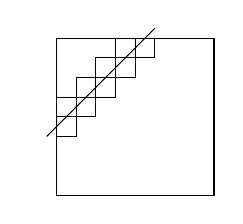
\begin{tikzpicture}[scale=0.25]
\draw (0,0) rectangle (8,8);
\begin{scope}[shift={(0,3)}]
\draw (-0.5,0) node[left] {$\calH$} -- (5,5.5);
\draw (0,0) rectangle (1,1) rectangle (2,2) rectangle (3,3) rectangle (4,4) rectangle (5,5);
\draw (0,1) rectangle (1,2) rectangle (2,3) rectangle (3,4) rectangle (4,5);
\end{scope}
\end{tikzpicture} &
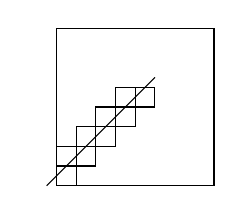
\begin{tikzpicture}[scale=0.25]
\draw (0,0) rectangle (8,8);
\begin{scope}%[shift={(0,3)}]
\draw (-0.5,0) node[left] {$\calH$} -- (5,5.5);
\draw (0,0) rectangle (1,1) rectangle (2,2) rectangle (3,3) rectangle (4,4) rectangle (5,5);
\draw (0,1) rectangle (1,2) rectangle (2,3) rectangle (3,4) rectangle (4,5);
\end{scope}
\end{tikzpicture} &
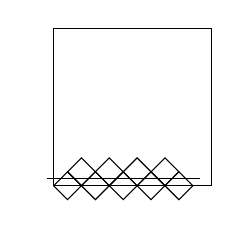
\begin{tikzpicture}[scale=0.25]
\draw (0,0) rectangle (8,8);
\begin{scope}[rotate=-45]
\draw (-0.5,0) node[left] {$\calH$} -- (5,5.5);
\draw (0,0) rectangle (1,1) rectangle (2,2) rectangle (3,3) rectangle (4,4) rectangle (5,5);
\draw (0,1) rectangle (1,2) rectangle (2,3) rectangle (3,4) rectangle (4,5);
\end{scope}
\end{tikzpicture}
\end{tabular}
\end{center}
Let $\beta\in\Part{\sigma}$ be $C\sigma$-close to $\calH$ and write $\beta=\beta'\times\beta_{d}$ with $\beta'\subset\R^{d-1}$ and $\beta_{d}\subset\R$.
Denote by $\Box(\beta)$ the box over $\beta$ as in \eqref{eq:Fourier-support}.
The crucial geometric obseravtion is that $\Box(\beta)$ is contained in a $C\sigma^{2}$-neighborhood of $\Box(\beta') \times \beta_{d}$.
Hence by \eqref{eq:dec-larger-Fourier-support} for each fixed $x_{d}\in\R$ we can apply the $(d-1)$-dimensional case of \eqref{eq:dec-const} to the functions $f_{\beta}(\cdot,x_{d},\cdot)$ of $d$ variables:
\[
\norm{ \sum_{\beta} f_{\beta}(\cdot,x_{d},\cdot) }_{L^{p}(\R^{d})}
\lesssim
\Dec^{p,2}_{d-1}(\sigma) \ell^{2}_{\beta} \norm{ f_{\beta}(\cdot,x_{d},\cdot) }_{L^{p}(\R^{d})}.
\]
By Minkowski's inequality it follows that
\begin{multline*}
\norm{ \sum_{\beta} f_{\beta} }_{L^{p}(\R^{d+1})}
=
L^{p}_{x_{d}\in\R} \norm{ \sum_{\beta} f_{\beta}(\cdot,x_{d},\cdot) }_{L^{p}(\R^{d})}
\lesssim
\Dec^{p,2}_{d-1}(\sigma) L^{p}_{x_{d}\in\R} \ell^{2}_{\beta} \norm{ f_{\beta}(\cdot,x_{d},\cdot) }_{L^{p}(\R^{d})}\\
\leq
\Dec^{p,2}_{d-1}(\sigma) \ell^{2}_{\beta} L^{p}_{x_{d}\in\R} \norm{ f_{\beta}(\cdot,x_{d},\cdot) }_{L^{p}(\R^{d})}
=
\Dec^{p,2}_{d-1}(\sigma) \ell^{2}_{\beta} \norm{ f_{\beta} }_{L^{p}(\R^{d+1})}.
\qedhere
\end{multline*}
\end{proof}


\subsubsection{Bourgain--Guth argument}\label{sec:gen:bourgain-guth}
We let $d\geq 1$ and assume that Theorem~\ref{thm:dec-paraboloid} holds with $d$ replaced by $d-1$.
In the case $d=1$ this hypothesis is vacuous.

From H\"older's inequality, it follows that
\begin{equation}\label{180713e3.4}
\MulDec_{d}^{p,2}(\delta, K)
\lesssim
\Dec_{d}^{p,2}(\delta).
\end{equation}
The Bourgain--Guth argument shows that the converse inequality also holds up to some lower-dimensional terms.
To be precise, we will prove
\begin{proposition}\label{prop:linear-vs-multilinear-dec}
Let $2 \leq p \leq 2(d+1)/(d-1)$.
Then for each $\epsilon>0$ there exists $K$ such that
\begin{equation}
\Dec_{d}^{p,2}(\delta)
\lesssim_{\epsilon}
\delta^{-\epsilon}
+ \delta^{-\epsilon} \max_{\delta\le \delta'\le 1; \delta' \text{dyadic}} \MulDec_{d}^{p,2}(\delta', K).
\end{equation}
\end{proposition}

Proposition~\ref{prop:linear-vs-multilinear-dec} is proved by iterating the following result $O(\frac{\abs{\log\delta}}{\log K})$ many times after choosing $K$ large enough depending on $\epsilon$ so that $C_{\epsilon} \leq K^{\epsilon}$.

\begin{proposition}
\label{prop:bourgain-guth-arg}
Let $2 \leq p \leq 2(d+1)/(d-1)$ and $\epsilon>0$.
Then for every $K$ that is a power of $4$ and $0<\delta<1/K$ we have
\begin{equation}
\label{eq:BG-arg}
\Dec_{d}^{p,2}(\delta)
\leq
C_{\epsilon} K^{\epsilon} \Dec_{d}^{p,2}(\delta K^{1/2})
+ C_{K} \MulDec_{d}^{p,2}(\delta, K).
\end{equation}
\end{proposition}
\begin{proof}[Proof of Proposition~\ref{prop:bourgain-guth-arg}]
Fix functions $f_{\theta}$, $\theta\in\Part{\delta}$.
Let $B \subset \R^{d+1}$ be a ball of radius $K$ and
\[
S_{B} := \Bigl( \sum_{\alpha\in\Part{K^{-1}}} \norm{f_{\alpha}}_{L^{p}(B)}^{2} \Bigr)^{1/2}.
\]
We distinguish two cases.
The first case is that there exists an affine hyperplane $\calH_{B}$ of $\R^{d}$ such that
\begin{equation}
\label{eq:small-away-from-hyperplane}
\norm[\Big]{ \sum_{\beta\in\Part{K^{-1/2}} : 2\beta \cap \calH_{B} = \emptyset} f_{\beta} }_{L^{p}(B)} \leq S_{B}.
\end{equation}
In this case we use Lemma~\ref{lem:hyperplane-dec} (for $d>1$; for $d=1$ triangle inequality suffices since there are only boundedly many summands in this case) and a simple localization argument as in Section~\ref{sec:dec-local} to obtain
\begin{multline*}
\norm[\Big]{ \sum_{\substack{\beta\in\Part{K^{-1/2}} \\ 2\beta \cap \calH_{B} \neq \emptyset}} f_{\beta} }_{L^{p}(B)}
\lesssim_{\epsilon}
K^{\epsilon} \Bigl( \sum_{\substack{\beta \in \Part{K^{-1/2}} \\ 2\beta \cap \calH_{B} \neq \emptyset}} \norm{ f_{\beta} }_{L^{p}(w_{B})}^{2} \Bigr)^{1/2}\\
\leq
K^{\epsilon} \Bigl( \sum_{\beta \in \Part{K^{-1/2}}} \norm{ f_{\beta} }_{L^{p}(w_{B})}^{2} \Bigr)^{1/2}.
\end{multline*}
If \eqref{eq:small-away-from-hyperplane} fails, then for every proper affine hyperplane $\calH$ of $\R^{d}$ there is a dyadic cube $\alpha \in \Part{K^{-1}}$ such that $\alpha$ is at least $K^{-1/2}$ away from $\calH$ and $\norm{f_{\alpha}}_{L^{p}(B)} \geq c_{K} S_{B}$.
We can therefore inductively choose such $\alpha_{1},\dotsc,\alpha_{d+1}$ in such a way that $\alpha_{k}$ is $K^{1/2}$ away from some affine hyperplane passing through $\alpha_{1},\dotsc,\alpha_{k-1}$.
In particular the collection $\alpha_{1},\dotsc,\alpha_{d+1}$ is $\nu_{K}$-transverse for some $\nu_{K}>0$ depending only on $d$ and $K$ and
\[
\norm{f}_{L^{p}(B)}
\leq
C_{K} S_{B}
\leq
C_{K} \avprod \norm{f_{\alpha_{i}}}_{L^{p}(B)},
\]
where $C_{K}$ are constants depending only on $d,K$.
Hence in both cases we obtain
\begin{multline*}
\norm{\sum_{\theta\in\Part{\delta}} f_{\theta}}_{L^{p}(B)}
\leq
\Bigl( \sum_{\alpha\in\Part{K^{-1}}} \norm{f_{\alpha}}_{L^{p}(B)}^{2} \Bigr)^{1/2}
+
C_{\epsilon} K^{\epsilon} \Bigl( \sum_{\beta \in \Part{K^{-1/2}}} \norm{ f_{\beta} }_{L^{p}(w_{B})}^{2} \Bigr)^{1/2}\\
+
C_{K} \sum_{\alpha_{1},\dotsc,\alpha_{d+1}\in\Part{K^{-1}}} \avprod \norm{f_{\alpha_{i}}}_{L^{p}(B)},
\end{multline*}
where the latter sum runs over all $\nu_{K}$-transverse tuples.
Replacing all $L^{p}(B)$ norms by averaged versions $\avL^{p}(B)$ and integrating this inequality over all $K$-balls $B\subset\R^{d+1}$ we obtain
\begin{align}
\notag
\norm{f}_{L^{p}(\R^{d+1})}
&=
L^{p}_{x \in \R^{d+1}} \norm{f}_{\avL^{p}(B(x,K))}\\
\label{eq:BG:small} & \leq
L^{p}_{x \in \R^{d+1}} \Bigl( \sum_{\alpha\in\Part{K^{-1}}} \norm{f_{\alpha}}_{\avL^{p}(B)}^{2} \Bigr)^{1/2}\\
\label{eq:BG:variety}&+
C_{\epsilon} K^{\epsilon} L^{p}_{x \in \R^{d+1}} \Bigl( \sum_{\beta \in \Part{K^{-1/2}}} \norm{ f_{\beta} }_{\avL^{p}(w_{B(x,K)})}^{2} \Bigr)^{1/2}\\
\label{eq:BG:transverse}&+
C_{K} \sum_{\substack{\alpha_{1},\dotsc,\alpha_{d+1}\in\Part{K^{-1}}\\\nu\text{-transverse}}} L^{p}_{x \in \R^{d+1}} \avprod \norm{f_{\alpha_{i}}}_{L^{p}(B(x,K))},
\end{align}
In the term \eqref{eq:BG:small}, by Minkowski's inequality and scaling we obtain 
\begin{align*}
\eqref{eq:BG:small}
&\leq
\Bigl( \sum_{\alpha\in\Part{K^{-1}}} (L^{p}_{x \in \R^{d+1}} \norm{f_{\alpha}}_{\avL^{p}(B)})^{2} \Bigr)^{1/2}\\
&=
\Bigl( \sum_{\alpha\in\Part{K^{-1}}} \norm{f_{\alpha}}_{L^{p}(\R^{d+1})})^{2} \Bigr)^{1/2}\\
&\leq
\Dec^{p,2}_{d}(\delta K) \Bigl( \sum_{\alpha\in\Part{\delta}} \norm{f_{\alpha}}_{L^{p}(\R^{d+1})})^{2} \Bigr)^{1/2}.
\end{align*}
The same argument is also applied to \eqref{eq:BG:variety}.
Note that by scaling $\Dec_{d}^{p,2}(\delta K) \leq \Dec_{d}^{p,2}(\delta K^{1/2})$, so the estimate for \eqref{eq:BG:small} can be absorbed in the estimate for \eqref{eq:BG:variety}.

In the last term \eqref{eq:BG:transverse} by definition of the multilinear decoupling constant \eqref{eq:multilin-Dec} we have
\begin{align*}
\eqref{eq:BG:transverse}
&\leq
C_{K} \MulDec^{p,2}_{d}(\delta,K) \sum_{\substack{\alpha_{1},\dotsc,\alpha_{d+1}\in\Part{K^{-1}}\\\nu\text{-transverse}}} \avprod \Bigl( \sum_{\theta\in\Part[\alpha_{i}]{\delta}} \norm{ f_{\theta} }_{L^{p}(\R^{d+1})}^{2} \Bigr)^{1/2}\\
&\leq
C_{K} \MulDec^{p,2}_{d}(\delta,K) \Bigl( \sum_{\theta\in\Part{\delta}} \norm{ f_{\theta} }_{L^{p}(\R^{d+1})}^{2} \Bigr)^{1/2},
\end{align*}
since $\Part[\alpha_{i}]{\delta} \subset \Part{\delta}$ and there are only $C_{K}$ choices of $\alpha_{1},\dotsc,\alpha_{d+1}$.
\end{proof}

% \end{document}
% \endinput
% \noindent\fbox{\parbox{\textwidth}{From here on this is a rough sketch}}

\subsection{Bourgain--Demeter iteration}
We will use two different moves to estimate the left-hand side of \eqref{eq:multilin-Dec}:
\begin{enumerate}
\item $L^{2}$ orthogonality.
This move allows to pull $\ell^{2}_{\tau}$ norms out of the inner $L^{p}$ norm.
This only works for $p=2$ and at an appropriate spatial scale given by the uncertainty principle.
\item Multilinear Kakeya.
This move allows to increase the radius of integration in the inner $L^{p}$ norm so that we have a chance of applying $L^{2}$ orthogonality again.
\end{enumerate}
These moves only work for specific combinations of Lebesgue exponents and scales.
\subsubsection{$L^2$ orthogonality}
\label{sec:L2-orth}
For every $0<\delta<1$ and every ball $B \subset \R^{d+1}$ of radius $\delta^{-1}$ we have
\begin{equation}\label{eq:L2-orth}
\norm[\Big]{\sum_{\theta\in\Part{\delta}}f_\theta }_{L^2(w_B)}
\lesssim
\ell^{2}_{\theta\in\Part{\delta}}\norm{f_\theta }_{L^2(w_B)}.
\end{equation}
It is important that this estimate holds already on balls of radius $\delta^{-1}$ given by the uncertainty principle.

To see \eqref{eq:L2-orth} let $\eta$ be a bump function adapted to the ball $B$ with $\abs{\eta} \sim 1$ on $B$.
Then
\[
\norm[\Big]{\sum_{\theta\in\Part{\delta}}f_\theta }_{L^2(B)}
\lesssim
\norm[\Big]{\sum_{\theta\in\Part{\delta}} \eta f_\theta }_{L^2(\R^{d+1})}
\lesssim
\ell^{2}_{\theta\in\Part{\delta}}\norm{\eta f_\theta }_{L^2(\R^{d+1})}
\lesssim
\ell^{2}_{\theta\in\Part{\delta}}\norm{f_\theta }_{L^2(w_{B})}
\]
by Plancherel's theorem, since the Fourier supports $\supp \widehat{\eta f_{\theta}}$ have bounded overlap (in fact, their projections onto $\R^{d}$ already have bounded overlap).
The estimate \eqref{eq:L2-orth} now follows from Lemma~\ref{lem:1-w}.

\subsubsection{Ball inflation}\label{sec:ball-inflation}
\begin{lemma}[Ball inflation, $\ell^{t}L^{t}$ version]
\label{lem:ball-inflation}
Let $0 < \rho \leq K^{-1}$.
Let $\alpha_1,\dotsc,\alpha_{d+1} \in \Part{K^{-1}}$ be a $\nu$-transverse collection of cubes.
Let $B\subset \R^{d+1}$ be a ball of radius $\rho^{-2}$.
Then for each $1 \leq t < \infty$ and $\epsilon>0$ we have
\begin{equation}\label{eq:ball-inflation:homogeneous}
\avL^{\frac{d+1}{d} t}_{x \in B} \avprod \ell^{t}_{\tau_i \in \Part[\alpha_i]{\rho}} \norm{f_{\tau_i}}_{\avL^{t}(w_{B(x,1/\rho)})}
\lesssim_{\nu,\epsilon} \rho^{-\epsilon}
\avprod \ell^{t}_{\tau_i \in \Part[\alpha_i]{\rho}} \norm{f_{\tau_i}}_{\avL^{t}(w_B)}.
\end{equation}
\end{lemma}

\begin{proof}
For each $\tau \in \Part{\rho}$ with center $c_{\tau}$ we cover $\R^{d+1}$ by a family $\Tubes_\tau$ of pairwise disjoint boxes (tubes) with $d$ short sides of length $\rho^{-1}$ and $1$ long side of length $\rho^{-2}$ pointing in the normal direction $N_{\mathbb{P}}(c_{\tau})$.
Let $\Tubes_{\tau}(B) := \Set{ T \in \Tubes_{\tau} \given T\cap B \neq \emptyset}$ and let $T_\tau(x) \in \Tubes_{\tau}$ denote the unique tube containing $x$.
By the multilinear Kakeya inequality (Corollary~\ref{cor:mult-Kakeya:functions}) we obtain
\begin{align*}
\MoveEqLeft
LHS\eqref{eq:ball-inflation:homogeneous}^{(d+1)t/d}\\
&=
\abs{B}^{-1} \int_{x\in B} \prod_{i=1}^{d+1} \Bigl( \sum_{\tau \in \Part[\alpha_{i}]{\rho}} \norm{f_{\tau}}_{\avL^{t}(w_{B(x,1/\rho)})}^{t} \Bigr)^{1/d}\\
&\lesssim_{\epsilon,\nu} \abs{B}^{-1} \rho^{-\epsilon} \rho^{-(d+1)}
\prod_{i=1}^{d+1} \Bigl( \sum_{\tau \in \Part[\alpha_{i}]{\rho}} \sum_{T\in \Tubes_{\tau}(B)} \sup_{x \in T} \norm{f_{\tau}}_{\avL^{t}(w_{B(x,1/\rho)})}^{t} \Bigr)^{1/d}\\
&\sim \rho^{-\epsilon}
\prod_{i=1}^{d+1} \Bigl( \sum_{\tau \in \Part[\alpha_{i}]{\rho}} \rho^{d} \sum_{T\in \Tubes_{\tau}(B)} \sup_{x \in T} \norm{f_{\tau}}_{\avL^{t}(w_{B(x,1/\rho)})}^{t} \Bigr)^{1/d}.
\end{align*}
To conclude the proof it remains to verify that
\[
\rho^{d} \sum_{T\in \Tubes_{\tau}(B)} \sup_{x \in T} \norm{f_{\tau}}_{\avL^{t}(w_{B(x,1/\rho)})}^{t}
\lesssim
\norm{f_{\tau}}_{\avL^{t}(w_{B})}^{t}.
\]
This inequality is morally true because each $f_{\tau}$ is constant at scale $1/\rho$ and the number of summands is of the order $\rho^{-d}$, so the left-hand side is a normalized $\avL^{t}$ norm.
We make this explanation precise.
Let $\psi_{\tau}$ be an $L^{1}$ normalized adapted bump function such that $f_{\tau} = f_{\tau} * \psi_{\tau}$.
Then
\begin{multline*}
\norm{ f_\tau  }_{\avL^t(w_{B(x, 1/\rho)})}^t
\sim
\rho^{d+1} \int \abs{f_\tau * \psi_{\tau}}^t(u) w_{B(x, 1/\rho)}(u) \dif u\\
\leq
\rho^{d+1} \norm{\psi_{\tau}}_{L^{1}}^{t-1}
\int (\abs{f_\tau}^{t} * \abs{\psi_{\tau}})(u) w_{B(x, 1/\rho)}(u) \dif u\\
\lesssim
\rho^{d+1} \int \abs{f_\tau}^{t}(u) (\abs{\psi_{\tau}}*w_{B(x, 1/\rho)})(u) \dif u.
\end{multline*}
For $x\in T \in \Tubes_{\tau}$ we have $\rho^{d+1} \abs{\psi_{\tau}}*w_{B(y, \rho^{-l})} \lesssim \tilde{w}_{T}$, where $\tilde{w}_{T}$ is an $L^{1}$ normalized bump function adapted to $T$, hence $\norm{\tilde{w}_{T}}_{\infty} \sim \rho^{d+2}$, so
\begin{multline*}
\rho^{d} \sum_{T\in \Tubes_{\tau}(B)} \sup_{x \in T} \norm{f_{\tau}}_{\avL^{t}(w_{B(x,1/\rho)})}^{t}
\lesssim
\rho^{d} \sum_{T\in \Tubes_{\tau}(B)} \int \abs{f_{\tau}}^{t} \tilde{w}_{T}\\
\lesssim
\rho^{2d+2} \int \abs{f_{\tau}}^{t} w_{B}
\sim
\norm{f_{\tau}}_{\avL^{t}(w_{B})}^{t}.
\qedhere
\end{multline*}
\end{proof}

\begin{corollary}[Ball inflation, $\ell^{q}L^{t}$ version]
\label{cor:ball-inflation:ell-r}
In the setting of Lemma~\ref{lem:ball-inflation} let $1 \leq q \leq t < \infty$.
Then
\begin{equation}\label{eq:ball-inflation:inhomogeneous}
\avL^{\frac{d+1}{d} t}_{x \in B} \avprod \ell^{q}_{\tau_i \in \Part[\alpha_i]{\rho}} \norm{f_{\tau_i}}_{\avL^{t}(w_{B(x,1/\rho)})}
\lesssim_{\nu,\epsilon} \rho^{-\epsilon}
\avprod \ell^{q}_{\tau_i \in \Part[\alpha_i]{\rho}} \norm{f_{\tau_i}}_{\avL^{t}(w_B)}.
\end{equation}
\end{corollary}

\begin{proof}
Let
\[
\calP_{i,l} := \Set[\Big]{ \tau \in \Part[\alpha_i]{\rho} \given 2^{-l-1} < \frac{\norm{f_{\tau}}_{\avL^{t}(w_B)}}{\max_{\tau' \in \Part[\alpha_i]{\rho}} \norm{f_{\tau'}}_{\avL^{t}(w_B)}} \leq 2^{-l}}
\]
and partition
\[
\Part[\alpha_{i}]{\rho} = \Bigl( \bigcup_{l=0}^{\tilde{l}} \calP_{i,l} \Bigr) \cup \calP_{i,\mathrm{rest}}
\]
with $\tilde{l} \sim \log \rho^{-1}$.
Then
\[
\ell^{q}_{\tau_i \in \Part[\alpha_i]{\rho}} \norm{f_{\tau_i}}_{\avL^{t}(w_{B(x,1/\rho)})}
\leq
\sum_{l_{i} \in \Set{0,\dotsc,\tilde{l}} \cup \Set{\mathrm{rest}}} \ell^{q}_{\tau_i \in \calP_{i,l_{i}}} \norm{f_{\tau_i}}_{\avL^{t}(w_{B(x,1/\rho)})},
\]
and since there are at most $C \log\rho^{-1}$ summands we may restrict the $\ell^{q}$ norm on the left-hand side of \eqref{eq:ball-inflation:homogeneous} to $\tau_{i} \in \calP_{i,l_{i}}$ for some choice of $l_{i} \in \Set{0,\dotsc,\tilde{l}} \cup \Set{\mathrm{rest}}$.
Since $q \leq t$, by H\"older's inequality and Lemma~\ref{lem:ball-inflation} we obtain
\begin{multline*}
\avL^{\frac{d+1}{d} t}_{x \in B} \avprod \ell^{q}_{\tau_i \in \calP_{i,l_{i}}} \norm{f_{\tau_i}}_{\avL^{t}(w_{B(x,1/\rho)})}\\
\leq
\bigl( \avprod \abs{\calP_{i,l_{i}}}^{1/q-1/t} \bigr) \avL^{\frac{d+1}{d} t}_{x \in B} \avprod \ell^{t}_{\tau_i \in \calP_{i,l_{i}}} \norm{f_{\tau_i}}_{\avL^{t}(w_{B(x,1/\rho)})}\\
\lesssim_{\nu,\epsilon} \rho^{-\epsilon}
\bigl( \avprod \abs{\calP_{i,l_{i}}}^{1/q-1/t} \bigr)
\avprod \ell^{t}_{\tau_i \in \calP_{i,l_{i}}} \norm{f_{\tau_i}}_{\avL^{t}(w_B)}.
\end{multline*}
It remains to show that
\[
\abs{\calP_{i,l}}^{1/q-1/t}
\ell^{t}_{\tau_i \in \calP_{i,l}} \norm{f_{\tau_i}}_{\avL^{t}(w_B)}
\lesssim
\ell^{q}_{\tau_i \in \Part[\alpha_{i}]{\rho}} \norm{f_{\tau_i}}_{\avL^{t}(w_B)}
\]
for every $l \in \Set{0,\dotsc,\tilde{l}} \cup \Set{\mathrm{rest}}$.
For $l \in \Set{0,\dotsc,\tilde{l}}$ we have in fact
\[
\abs{\calP_{i,l}}^{1/q-1/t}
\ell^{t}_{\tau_i \in \calP_{i,l}} \norm{f_{\tau_i}}_{\avL^{t}(w_B)}
\sim
\abs{\calP_{i,l}}^{1/q} \max_{\tau_i \in \calP_{i,l}} \norm{f_{\tau_i}}_{\avL^{t}(w_B)}
\sim
\ell^{q}_{\tau_i \in \calP_{i,l}} \norm{f_{\tau_i}}_{\avL^{t}(w_B)},
\]
while for $l=\mathrm{rest}$ we have
\[
\abs{\calP_{i,\mathrm{rest}}}^{1/q-1/t}
\ell^{t}_{\tau_i \in \calP_{i,\mathrm{rest}}} \norm{f_{\tau_i}}_{\avL^{t}(w_B)}
\lesssim
\abs{\Part[\alpha_{i}]{\rho}}^{1/q} 2^{-\tilde{l}}
\max_{\tau' \in \Part[\alpha_{i}]{\delta}} \norm{f_{\tau'}}_{\avL^{t}(w_B)},
\]
and the claim follows provided that $\tilde{l}$ is a sufficienly large multiple of $\log \rho^{-1}$.
\end{proof}

\subsubsection{Proof of Theorem~\ref{thm:dec-paraboloid} for $p=2\frac{d+1}{d}$}
The proof of Theorem~\ref{thm:dec-paraboloid} in the range $2 \leq p \leq 2\frac{d+1}{d}$ is easier than in the general case and also historically it appeared earlier \cite{MR3038558}.
By interpolation it suffices to consider $p=2\frac{d+1}{d}$.

In view of Proposition~\ref{prop:linear-vs-multilinear-dec} it suffices to estimate the multilinear decoupling constant.
Throughout this section let $\alpha_1,\dotsc,\alpha_{d+1} \in \Part{K^{-1}}$ be $\nu_{K}$-transverse cubes.
For $\rho \in 2^{-\N}$ we define the quantity
\begin{equation}\label{eq:Bourgain-Demeter-A}
A(\rho)
:=
L^{p}_{x} \avprod \ell^{2}_{\tau\in \Part[\alpha_i]{\rho}} \norm{f_{\tau}}_{\avL^{2}(w_{B(x,1/\rho)})}.
\end{equation}
We caution the reader that the quantities denoted by $A$ in \cite{MR3592159} would correspond to our $A$ with $L^{p}_{x}$ replaced by $\avL^{p}_{x\in B}$ for a large ball $B$.

\begin{proposition}
\label{prop:iter:low-p}
We have for $p = 2 \frac{d+1}{d}$ and $\epsilon>0$
\begin{equation}
\label{eq:iter:low-p}
A(\rho)
\lesssim_{K,\epsilon}
\rho^{-\epsilon} A(\rho^{2})
\end{equation}
\end{proposition}
\begin{proof}
Using ball inflation (Lemma~\ref{lem:ball-inflation}) with $t=2$ we obtain
\begin{align*}
A(\rho)
&=
L^{p}_{x} \avL^{p}_{\tilde{x} \in B(x,1/\rho^{2})} \avprod \ell^{2}_{\tau\in \Part[\alpha_i]{\rho}} \norm{f_{\tau}}_{\avL^{2}(w_{B(\tilde{x},1/\rho)})}\\
&\lesssim_{K,\epsilon} \rho^{-\epsilon}
L^{p}_{x} \avprod \ell^{2}_{\tau\in \Part[\alpha_i]{\rho}} \norm{f_{\tau}}_{\avL^{2}(w_{B(x,1/\rho^{2})})}
\end{align*}
By $L^{2}$ orthogonality we have
\begin{equation}\label{eq:L2-orth-scale-rho^2}
\norm{f_{\tau}}_{\avL^{2}(w_{B(x,1/\rho^{2})})}
\lesssim
\ell^{2}_{\tau' \in \Part[\tau]{\rho^{2}}}\norm{f_{\tau'}}_{\avL^{2}(w_{B(x,1/\rho^{2})})},
\end{equation}
and the conclusion follows.
\end{proof}
Now we relate the quantity $A$ with the multilinear decoupling inequality.
Let $\rho \leq (2K)^{-1}$.
Then
\begin{equation}\label{eq:triv-est-by-A}
\begin{split}
LHS\eqref{eq:multilin-Dec}
&=
L^{p}_{x} \avL^{p}_{\tilde{x} \in B(x,1/(2\rho))} \avprod \norm{f_{\alpha_i}}_{\avL^p(B(\tilde{x},K))}\\
\text{by H\"older }&\leq
L^{p}_{x} \avprod \avL^{p}_{\tilde{x} \in B(x,1/(2\rho))} \norm{f_{\alpha_i}}_{\avL^p(B(\tilde{x},K))}\\
&\lesssim
L^{p}_{x} \avprod \norm{f_{\alpha_i}}_{\avL^p(B(x,1/\rho))}\\
\text{by Minkowski}&\leq
L^{p}_{x} \avprod \ell^{1}_{\theta\in\Part[\alpha_i]{\rho}} \norm{f_{\theta}}_{\avL^p(B(x,1/\rho))} \\
\text{by H\"older }&\leq
\rho^{-d/2}
L^{p}_{x} \avprod \ell^{2}_{\theta\in\Part[\alpha_i]{\rho}} \norm{f_{\theta}}_{\avL^p(B(x,1/\rho))}\\
\text{by reverse H\"older}&\lesssim
\rho^{-d/2}
L^{p}_{x} \avprod \ell^{2}_{\theta\in\Part[\alpha_i]{\rho}} \norm{f_{\theta}}_{\avL^2(w_{B(x,1/\rho)})}\\
&=
\rho^{-d/2}
A(\rho)
\end{split}
\end{equation}
On the other hand, for any $\rho$ by H\"older's and Minkowski's inequalities we obtain
\begin{multline}
\label{eq:trivial-est-for-A}
A(\rho)
\leq
\avprod L^{p}_{x} \ell^{2}_{\tau\in \Part[\alpha_i]{\rho}} \norm{f_{\tau}}_{\avL^{p}(w_{B(x,1/\rho)})}
\leq
\avprod \ell^{2}_{\tau\in \Part[\alpha_i]{\rho}} L^{p}_{x} \norm{f_{\tau}}_{\avL^{p}(w_{B(x,1/\rho)})}\\
\sim
\avprod \ell^{2}_{\tau\in \Part[\alpha_i]{\rho}} \norm{f_{\tau}}_{L^{p}(\R^{d+1})}.
\end{multline}
Using \eqref{eq:triv-est-by-A}, iterating \eqref{eq:iter:low-p} $m$ times, and using \eqref{eq:trivial-est-for-A} at the end we obtain for $\delta = \rho^{2^{m}}$ the estimate
\[
LHS~\eqref{eq:multilin-Dec}
\lesssim_{K,m,\epsilon} \rho^{-d/2} \rho^{-\epsilon} \dotsm \rho^{-2^{m-1}\epsilon}
\avprod \ell^{2}_{\theta\in \Part[\alpha_i]{\delta}} \norm{f_{\theta}}_{L^{p}(\R^{d+1})},
\]
so that
\[
\MulDec^{p,2}_{d}(\delta,K) \lesssim_{K,m,\epsilon} \delta^{-d 2^{-m+1}-\epsilon}.
\]
Choosing $m$ large enough this gives $\MulDec^{p,2}_{d}(\delta,K) \lesssim_{K,\epsilon} \delta^{-\epsilon}$, and this suffices to conclude the proof of Theorem~\ref{thm:dec-paraboloid}.


\subsubsection{Proof of Theorem~\ref{thm:dec-paraboloid} for $p=2\frac{d+2}{d}$}
For $p > 2 \frac{d+1}{d}$ we will have to apply ball inflation with some $t>2$.
This necessitates some additional branching of the estimates since orthogonality is only available in $L^{2}$.
\begin{proposition}
\label{prop:iter}
We have for $p = 2\frac{d+2}{d}$ and $\epsilon>0$
\begin{equation}
\label{eq:iter:high-p}
A(\rho)
\lesssim_{K,\epsilon}
\rho^{-\epsilon} A(\rho^{2})^{1/2}
\Bigl( \Dec_{d}^{p,2}(\delta/\rho) \avprod \ell^{2}_{\theta \in \Part[\alpha_i]{\delta}} \norm{ f_{\theta} }_{p} \Bigr)^{1/2}
\end{equation}
\end{proposition}
\begin{proof}
Using ball inflation (Corollary~\ref{cor:ball-inflation:ell-r}) with $q=2$ and $t=p d/(d+1)$ we obtain
\begin{align*}
A(\rho)
&=
L^{p}_{x} \avL^{p}_{\tilde{x} \in B(x,1/\rho^{2})} \avprod \ell^{2}_{\tau\in \Part[\alpha_i]{\rho}} \norm{f_{\tau}}_{\avL^{2}(w_{B(\tilde{x},1/\rho)})}\\
\text{by H\"older } &\lesssim
L^{p}_{x} \avL^{p}_{\tilde{x} \in B(x,1/\rho^{2})} \avprod \ell^{2}_{\tau\in \Part[\alpha_i]{\rho}} \norm{f_{\tau}}_{\avL^{t}(w_{B(\tilde{x},1/\rho)})}\\
\text{by Cor.~\ref{cor:ball-inflation:ell-r} } &\lesssim_{K,\epsilon} \rho^{-\epsilon}
L^{p}_{x} \avprod \ell^{2}_{\tau\in \Part[\alpha_i]{\rho}} \norm{f_{\tau}}_{\avL^{t}(w_{B(x,1/\rho^{2})})}\\
\text{by H\"older } &\leq \rho^{-\epsilon}
\Big( L^{p}_{x} \avprod \ell^{2}_{\tau\in \Part[\alpha_i]{\rho}} \norm{f_{\tau}}_{\avL^{2}(w_{B(x,1/\rho^{2})})} \Big)^{1/2}\\
&\quad\cdot
\Big( L^{p}_{x} \avprod \ell^{2}_{\tau\in \Part[\alpha_i]{\rho}} \norm{f_{\tau}}_{\avL^{p}(w_{B(x,1/\rho^{2})})} \Big)^{1/2}.
\end{align*}
Here we used $1/t = (1/2)(1/2) + (1/2)(1/p)$.
By $L^{2}$ orthogonality \eqref{eq:L2-orth-scale-rho^2} the first bracket is $\lesssim A(\rho^{2})$.
In the second bracket we estimate
\begin{equation}
\label{eq:37}
\begin{split}
&
L^{p}_{x} \avprod \ell^{2}_{\tau\in \Part[\alpha_i]{\rho}} \norm{f_{\tau}}_{\avL^{p}(w_{B(x,1/\rho^2)})}\\
\text{by H\"older }&\leq
\avprod L^{p}_{x} \ell^{2}_{\tau\in \Part[\alpha_i]{\rho}} \norm{f_{\tau}}_{\avL^{p}(w_{B(x,1/\rho^2)})}\\
\text{by Minkowski }&\leq
\avprod \ell^{2}_{\tau\in \Part[\alpha_i]{\rho}} L^{p}_{x} \norm{f_{\tau}}_{\avL^{p}(w_{B(x,1/\rho^2)})}\\
&\lesssim
\avprod \ell^{2}_{\tau\in \Part[\alpha_i]{\rho}} \norm{f_{\tau}}_{p}\\
\text{by scaling }&\lesssim
\avprod \ell^{2}_{\tau\in \Part[\alpha_i]{\rho}} \bigl( \Dec_{d}^{p,2}(\delta/\rho) \ell^{2}_{\theta\in \Part[\tau]{\delta}} \norm{f_{\theta}}_{p} \bigr)\\
&=
\Dec_{d}^{p,2}(\delta/\rho) \avprod \ell^{2}_{\theta\in \Part[\alpha_i]{\delta}} \norm{f_{\theta}}_{p}.
\qedhere
\end{split}
\end{equation}
\end{proof}

\begin{lemma}\label{lem:bourgain-demeter}
Let $p = 2\frac{d+2}{d}$ and suppose that
\begin{equation}
\label{eq:40}
\Dec^{p,2}_{d}(\delta) \leq C \delta^{-\eta}
\end{equation}
for some $0<\eta<\infty$ and some $0<C<\infty$.
Then for every $K$ we have
\[
\MulDec^{p}(\delta,K) \lesssim_{K,\eta, C} \delta^{-\eta(1-2^{-d/\eta-1})}.
\]
\end{lemma}
\begin{proof}
Choose $\nu_{K}$-transverse $\alpha_{1},\dotsc,\alpha_{M} \in \Part{1/K}$.
Choose functions $f_{\theta}$ with
\[
\ell^{2}_{\theta \in \Part[\alpha_i]{\delta}} \norm{f_\theta}_{p} = 1.
\]
Let $m\in\N$ be chosen later.
Using \eqref{eq:triv-est-by-A}, iterating \eqref{eq:iter:high-p} $m$ times, and using \eqref{eq:trivial-est-for-A} at the end we obtain for $\delta = \rho^{2^{m}}$ the estimate
\begin{align*}
LHS~\eqref{eq:multilin-Dec}
&\lesssim_{m,K,\epsilon}
\rho^{-d/2}
\prod_{l=0}^{m-1} \Bigl( \rho^{-2^{l}\epsilon} \Dec(\delta/\rho^{2^{l}})^{1/2} \Bigr)^{2^{-l}}\\
&\lesssim
\rho^{-d/2} \prod_{l=0}^{m-1} (\delta/\rho^{2^{l}})^{-2^{-l-1}\eta} \rho^{-\epsilon}\\
&=
\rho^{-d/2-m\epsilon} \prod_{l=0}^{m-1} \rho^{\eta/2} \delta^{-2^{-l-1}\eta}\\
&=
\rho^{-d/2-m\epsilon+m\eta/2} \delta^{-(1-2^{-m})\eta}.
\end{align*}
If $m\eta > d$ and $\epsilon$ is small enough, then this is $\leq \delta^{-(1-2^{-m})\eta}$, and the claim follows.
\end{proof}

Now we conclude the proof of Theorem~\ref{thm:dec-paraboloid} for $p = 2\frac{d+2}{d}$.
If is easy to see that
\begin{equation}\label{eq:dec-exponent}
\Dec^{p,2}_{d}(\delta) \lesssim \delta^{-\eta}
\end{equation}
for some $\eta<\infty$.
Suppose that \eqref{eq:dec-exponent} holds for some $\eta>0$.
We will decrease $\eta$.
Substituting the conclusion of Lemma~\ref{lem:bourgain-demeter} into the conclusion of Proposition~\ref{prop:linear-vs-multilinear-dec} gives
\begin{equation}\label{eq:dec-exponent:improved}
\Dec^{p,2}_{d}(\delta)
\lesssim_{\epsilon} \delta^{-\epsilon}
+
\delta^{-\epsilon- (1 - 2^{-d/\eta-1}) \eta}
\end{equation}
for any $\epsilon>0$.
Iterating the passage from \eqref{eq:dec-exponent} to \eqref{eq:dec-exponent:improved} we can make $\eta$ arbitrarily close to $0$.
